\chapter[Gemeinsamkeiten und Unterschiede]{Gemeinsamkeiten und Unterschiede von SOA und Microservices}
\label{chap:Unterschiede}
%Einsatzmöglichkeiten!!!! 
% - nötigen Architekturen und Schnittstellen 
% - Plattformen und Voraussetzungen für den Einsatz der jeweiligen Paradigmen

%Vor- und Nachteile der Paradigmen, 
% - Prozessisolierung
% - Skalierung
% - Deployment
% - Wartbarkeit (insbesondere der Korrigierbarkeit, Erweiterbarkeit, Anpassbarkeit, Verbesserung)
% - Entwicklung/Testbarkeit 
% - Bindung an Technologie-Stacks
\section{Einsatzgebiet}
\label{sec:Einsatzgebiet}
Sowohl SOA, als auch Microservices sind Paradigmen aus der Service-orientierten Architektur, verfolgen jedoch unterschiedliche Ansätze. Während das Microservice-Paradigma die Softwareentwicklungsabteilung unterstützen soll, soll mit Hilfe von SOA die Kommunikation zwischen den Anwendungen und den Abteilungen standardisiert und optimiert werden.
\\\\
Mit Hilfe des Microservice Paradigmas wird die Struktur einer Anwendung in mehrere, kleinere Dienste aufgeteilt. Dadurch ist es möglich neue Technologien einzusetzen und gegebenenfalls zu ersetzten, sollten diese nicht den gewünschten Erfolg bringen.
\\\\
Anders sieht es mit SOA aus. Hierbei werden Adapter für Anwendungen, wie Kommerzielle Systeme oder Eigenentwicklungen, entwickelt, welche zusammen mit der Anwendung als Dienst dienen. Der Adapter stellt eine Schnittstelle für die Funktionalität der Anwendung bereit und übernimmt das steuern der Anwendung und das abfangen von Fehleingaben.

\begin{quotation}
	\frqq Aber der wichtigste Unterschied zwischen SOA und Microservices ist die Ebene, auf der die Architekturen ansetzen. Die Architektur einer SOA betrachtet das gesamte Unternehmen, SOA definiert, wie eine Vielzahl von Systemen in der Enterprise-IT interagieren. Microservices hingegen sind eine Architektur für ein einzelnes System. Sie sind eine Alternative zu anderen Modularisierungstechnologien. [..] Eine vollständige SOA umfasst die gesamte Unternehmens-IT.\flqq\ \cite[S. 90]{EWolff2016:Microservices}
\end{quotation}

\section{Architekturen und Schnittstellen}
\label{sec:ArchitekturenUndSchnittstellen}
Beide Paradigmen sind Service-orientierte Systeme, welche auf ein verteiltes System setzten. Dabei existiert eine beliebige Anzahl verschiedener Dienste, welche verschiedene Funktionalitäten bereitstellen. Damit der Ausfall eines Dienstes, keine weiteren Dienste direkt beeinflusst, werden diese oft in eigenen Umgebungen, wie virtuelle Maschinen, betrieben. 

\begin{quotation}
	\frqq Microservices sollen unabhängig voneinander in Produktion gebracht werden [..]. Daher ist jeder Microservice meistens auf einem eigenen Server beheimatet.\flqq\ \cite[S. 80]{EWolff2016:Microservices}
\end{quotation}

Bei SOA sollten die einzelnen Services, ebenfalls auf eigenen Servern beheimatet sein, um eine Unabhängigkeit zu anderen Services zu gewährleisten.
\\\\
Während bei SOA eine zentrale Kommunikationseinheit (der ESB) existiert, sind Microservices in der Kommunikation frei. Dies bedeutet, dass der ESB in einem SOA-System entsprechende Werte oder Fehlermeldungen zurückgeben kann, während Microservices selber auf fehlgeschlagene Anfragen reagieren muss.

\begin{quotation}
	\frqq In einer SOA ist die Integrationslösung auch für die Orchestrierung der Services zuständig. Ein Geschäftsprozess wird aus den Services zusammengestellt. In einer Microservice-Architektur besitzt die Integrationslösung keine eigene Intelligenz. Die Microservices sind dafür zuständig, mit den anderen Services zu kommunizieren.\flqq\ \cite[S. 89]{EWolff2016:Microservices}
\end{quotation}

Damit Dienste untereinander kommunizieren können, sind Schnittstellen (APIs) notwendig, über welche die Informationen abgefragt bzw. bereitgestellt werden können. Da jedoch in einem SOA-System ganze Applikationen verwendet werden, ist es oft notwendig, zunächst einmal zu entscheiden, wie dessen Funktionalitäten angeboten werden sollen.
\\\\
Zum einen können Adapter verwendet werden, die jegliche Informationen der Anwendung bereitstellen. Dadurch ist es möglich durch Standardisierte Verfahren wie SOAP/HTTP oder REST/HTTP den Dienst wiederzuverwenden.
\\\\
Zum anderen bedeutet diese Aufteilung, dass oft eine große Menge an Informationen abgefragt werden. Dies macht gegenüber dem Business kein Sinn, da zum Teil unnötig viele Informationen für die nächste Generation von Anwendungen bereitgestellt werden. In diesem Fall werden "`Service Komponenten"' verwendet, welche als Adapter dienen und die benötigten Informationen aus den Applikationen abfragen und bereitstellen.
\begin{quotation}
	\frqq SOA führt nur eine neue Schicht über den vorhandenen Services ein, um die Anwendungen neu zu kombinieren. Es zielt auf eine flexible Integration der vorhandenen Anwendungen.\flqq\ \cite[S. 92]{EWolff2016:Microservices}
\end{quotation}

\begin{figure}[htb]
    \centering 
    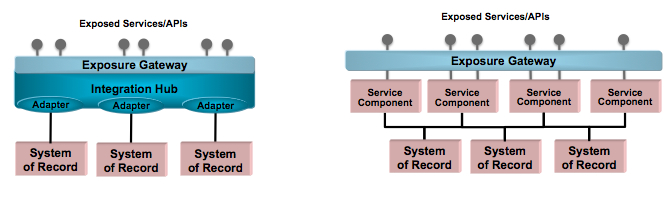
\includegraphics[width=\linewidth]{content/images/figure2}\
    \quelle\url{https://www.ibm.com/developerworks/websphere/library/techarticles/1601_clark-trs/1601_clark.html} (Stand 16.12.2016)
    \caption{Technische und Funktionale Sicht von SOA}
    \label{fig:TechnicalAndFunctionalViewsOfSOA} 
\end{figure}

In einer Microservice-Architektur, besitzt ein Microservice nur eine Aufgabe und ist dadurch deutlich kleiner, als ein Service in einer SOA-Architektur, bei dem der Service aus einer monolithischen Anwendung, mit entsprechenden Schnittstellen, besteht.
\begin{figure}[htb]
    \centering 
    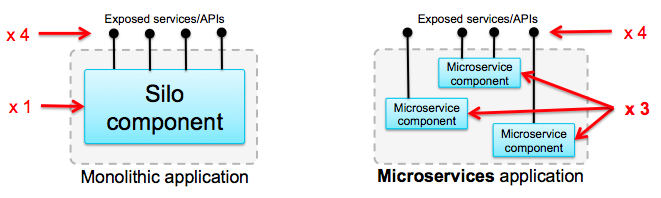
\includegraphics[width=\linewidth]{content/images/MonolithicVsMicroservice}\
    \quelle\url{https://www.ibm.com/developerworks/websphere/library/techarticles/1601_clark-trs/1601_clark.html} (Stand 16.12.2016)
    \caption{Monolithische vs Microservice Applikation}
    \label{fig:MonolithicVsMicroservice} 
\end{figure}
\newpage
Dies bedeutet jedoch häufig, dass weitere Microservices notwendig sind, um Informationen zusammen zu führen. Dadurch ergibt sich ein Geflecht aus Microservices, welche untereinander kommunizieren und zum Teil aufeinander angewiesen sind.
\\\\
Da in einer SOA-Architektur, als auch in einer Microservice-Architektur, die Services Schnittstellen anbieten müssen, damit diese über das Netzwerk angesprochen werden können. Muss dafür gesorgt werden, dass die Interoperabilität, mit Hilfe der Schnittstellen, gewährleistet wird.
\\\\
Dadurch, dass die Kommunikation über Schnittstellen erfolgt, kann, sofern diese Standardisiert sind und Beispielsweise als SOAP/HTTP oder REST/HTTP umgesetzt wurden, der Dienst Plattform unabhängig deployed werden. Da jedoch monolithische Anwendungen oft sehr umfangreich sind, werden diese meistens für ein bestimmtes Betriebssystem gebaut. Microservices hingegen sind kleine autarke Dienste, Dadurch ist es möglich diese Plattform unabhängig zu deployen. Hier drauf wird in weiter unten, unter \ref{subsec:BindungAnTechnologiestacks} \nameref{subsec:BindungAnTechnologiestacks}, genauer eingegangen.

\section{Vor- und Nachteile}
\label{sec:VorUndNachteile}

\subsection{Prozessisolierung}
\label{subsec:Prozessisiolierung}
Ein wichtiger Grundsatz von Service-orientierten Systemen ist, dass Dienste autark bleiben. Um dies zu erreichen, darf nur eine lose Kopplung zwischen einzelne Dienste stattfinden. Dies wird durch Zustandslose Schnittstellen und Eigenständigkeit erreicht. Damit ist gemeint, dass jeder Dienst seine Aufgaben, zum größten Teil alleine durchführen kann ohne auf andere Dienste angewiesen zu sein.
\\\\
Eine Vollständige Autarkheit ist in einem Microservice System nicht möglich. Trotzdem wird versucht Aufgaben möglichst zu Isolieren.

\begin{quotation}
	\frqq Microservices setzten auf Isolation: Idealerweise wird eine Benutzerinteraktion vollständig in einem Microservice abgearbeitet und es ist kein Aufruf eines anderen Microservices notwendig.\flqq\ \cite[S. 90]{EWolff2016:Microservices}
\end{quotation}

Folgende Abbildung zeigt jedoch, dass eine vollständige Isolation, häufig nicht möglich ist. Da Microservices klein sein und nur eine Aufgabe erledigen sollen, müssen häufig weitere Microservices verwendet werden, um eine komplexe Aufgabe zu erledigen.

\begin{figure}[htb]
    \centering 
    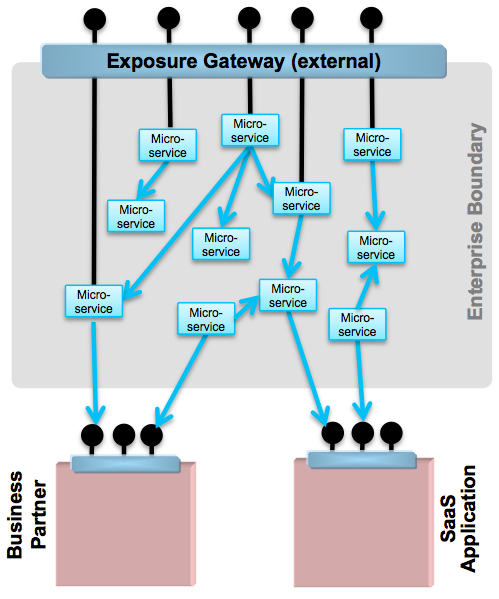
\includegraphics[width=300px]{content/images/figure6}\
    \quelle\url{https://www.ibm.com/developerworks/websphere/library/techarticles/1601_clark-trs/1601_clark.html} (Stand 16.12.2016)
    \caption{Microservice Architektur}
    \label{fig:MicroserviceArchitekturInGreenField} 
\end{figure}
\newpage
Bei SOA hingegen besteht ein Dienst, wie bereits in \ref{sec:UnternehmensKomponenten} \nameref{sec:UnternehmensKomponenten} erwähnt, aus einer vollständigen Anwendung und einem Adapter, welcher die Steuerung der Anwendung über APIs bereitstellt. Dadurch, dass eine Anwendung alle nötigen Fachlichkeiten und Ressourcen, für die Ausführung der Anwendung besitzt, ist der Dienst vollständig Autark. Lediglich die Frontend-Anwendungen sind auf die APIs und damit auf die Backend-Anwendungen angewiesen. Fällt zum Beispiel eine Anwendung aus, kann es dazu führen, dass das gesamte System nicht mehr funktioniert, da die Dienste häufig in eine Wertschöpfungskette eingebunden sind.

\subsection{Deployment}
\label{subsec:Deployment}
Das Deployment ist in einem Service-orientiertem System von entscheidender Bedeutung und darf nicht unterschätzt werden. Oft werden Continuous Deployment Pipelines aufgebaut, um diesen Prozess zu automatisieren. Innerhalb der Pipeline wird sowohl die Umgebung, in welcher der Dienst später laufen soll, aufgebaut, sowie der Dienst in die zuvor, vorbereitete Umgebung deployed. Unter Umständen ist ein erneutes Deployen notwendig, wenn sich die Anforderungen an einen Dienst geändert haben oder Fehler behoben wurden. Dabei stellt das Deployment eine besondere Herausforderung dar. 

\begin{quotation}
	\frqq Das Deployment wäre zwar unabhängig voneinander möglich, aber die Test-Stages vor dem Deployment müssen immer noch koordiniert und von jeder Änderung einzeln durchlaufen werden.\flqq\ \cite[S. 19]{EWolff2016:Microservices}
\end{quotation}

Dadurch, dass Microservices kleine autarke Dienste sind, ist es oft nicht nötig, viele Konfigurationsdateien anzupassen bzw. bereitzustellen. Jedoch sind oft eine Vielzahl von Microservices in einem System vorhanden und müssen deployed, sowie gemanagt werden.

\begin{quotation}
	\frqq Durch die Umsetzung der Microservices entsteht zunächst zusätzliche Komplexität: Die vielen Micorservices benötigen eigene Infrastrukturen\flqq\ \cite[S. 18]{EWolff2016:Microservices}
\end{quotation}

Dienste in einem SOA-System hingegen sind häufig ganze Anwendungen. Diese erfordern oft eine aufwändige Konfiguration, welche nicht immer mit Hilfe von Konfigurationsdateien vorgenommen werden können. Einige Anwendungen dürfen nur durch den Hersteller oder durch ihn Zertifizierte Unternehmen Installiert und/oder Konfiguriert werden. Dadurch ist ein automatisches Deployment nicht möglich und auch ein manuelles Deployment wird erschwert.

\subsection{Skalierung}
\label{subsec:Skalierung}
Nicht immer können stark genutzte Anwendungen, durch Aufwertung oder Erweiterung von Hardware, belastbarer gemacht werden. Kritische oder Zentrale Anwendungen eines Unternehmens sind nicht nur stark genutzt, sondern dürfen nicht ausfallen. Durch Hardware, kann nicht durchgängig sichergestellt werden, dass eine Anwendung erreichbar ist. Um diese Problematiken entgegen zu wirken, muss Skaliert werden. Dabei werden mehrere Instanzen eines Systems parallel betrieben.

\begin{quotation}
	\frqq Skalierbarkeit bedeutet nur, dass die Last auf mehrere Knoten verteilt werden kann. Wie das System tatsächlich auf Last reagiert, ist offen. Wichtiger ist eigentilch, dass sich das System tatsächlich einer steigenden last anpasst. Dazu ist es notwendig, dass ein Microservice abhängig von der Last neue Instanzen starten, auf die Last verteilt werden kann.\flqq\ \cite[S. 151]{EWolff2016:Microservices}
\end{quotation}

In einem Microservice-System, ist es möglich, in kürzester Zeit eine weitere Instanz eines Dienstes zu starten und zu betreiben. Dadurch kann in kürzester Zeit auf verschiedene Lasten von Diensten reagiert werden, ohne dass ein Mensch in das System eingreifen muss. Es ist bei einem Microservice-System möglich, wenig genutzte Dienste, nur bei Bedarf zu starten und nach einer gewissen Zeit der Inaktivität, zu stoppen. Kritische oder stark genutzte Dienste hingegen, besitzen meistens mehrere Instanzen, auf denen die Lasten verteilt werden. Dadurch wird ebenfalls eine Ausfallsicherheit gewährleistet.
\\\\
SOA-Systeme besitzen deutlich größere Dienste als Microservice-Systeme. Existiert kein standardisiertes und automatisiertes Konfigurationsmanagement, stellt sich die Skalierung von monolithischen Anwendungen, als schwieriger heraus, da häufig viele Einstellungen und Installationen manuell vorgenommen werden müssen. Dadurch ist eine einfache Skalierung nicht möglich. Daher werden häufig, weitere Instanzen, dauerhaft parallel betrieben, um die Last auf mehrere Instanzen zu verteilen. Sind monolithische Anwendungen nicht Zustandslos, wird dadurch das Skalieren ebenfalls erschwert.

\subsection{Wartbarkeit}
\label{subsec:Wartbarkeit}
Im Laufe der Zeit wachsen die Anforderungen an einen Dienst, wodurch dieser angepasst, verbessert oder erweitert werden muss. Zur Wartung gehört jedoch auch das korrigieren von Fehlern, welches einer der einfachsten Aufgaben in einem Service-orientierten System ist, da sich dadurch meistens, nicht die Schnittstellen, Umgebung oder die Konfiguration des Dienstes ändert. Anders sieht dies jedoch beim Anpassen, Verbessern oder Erweitern aus.
\\\\
Das Anpassen einer Anwendung kann sich von dem Verbessern oder Erweitern einer Anwendung unterscheiden. Zum Beispiel reicht es aus die Mehrwertsteuer in einer Anwendung zu ändern, welches eine Anpassung darstellt, jedoch keine Verbesserung oder Erweiterung. Das Anpassen ist durch die kaum veränderten Strukturen relativ leicht. Anders sieht dies jedoch bei Verbesserungen oder Erweiterungen aus. Beide Änderungen sorgen für eine Veränderung der internen Struktur des Quelltextes. Zusätzlich ist man an den vorgegebenen Technologie-Stacks gebunden. Oft sind Verbesserungen oder Erweiterungen nicht ohne das Verändern der Quelltextstruktur möglich.
\\\\
Während in einem SOA-System der Dienst aus einer Anwendung und einem Adapter besteht und damit ein fast monolithisches System abbildet. Besteht ein Microservice-System aus viele unterschiedlichen Diensten. In beiden Systemen ist es möglich, in kürzester Zeit Fehler zu korrigieren, sofern die nötigen Voraussetzungen gegeben sind. Das Anpassen, Verbessern oder Erweitern eines Dienstes, gestaltet sich jedoch einfacher in einem Microservice-System, als in einem SOA-System. Aufgrund der Größe von Microservices, kann ein Microservice von Grund auf neu erstellt werden, sollte dies nötig sein. Muss das System erweitert werden, können neue Microservices erstellt, welche die neuen Anforderungen bzw. Fachlichkeiten abbilden. Durch die Autarkheit von Microservices, können diese deployed werden, ohne die Interoperabilität des bestehenden Systems zu gefährden oder zu beeinflussen. Anschließend müssen gegebenenfalls einzelne Dienste angepasst werden, um die neuen Funktionalitäten, in das bestehende System, einzubinden.

\subsection{Bindung an Technologie-Stacks}
\label{subsec:BindungAnTechnologiestacks}
In beiden Paradigmen, sollten Dienste eine standardisierte Schnittstelle besitzen, damit diese, durch andere Dienste verwendet werden können. Zusätzlich ist dadurch eine Wiederverwendung des Dienstes möglich. Das verwenden einer standardisierten Schnittstelle schränkt jedoch die Auswahl der einzusetzenden Technologien ein. Zudem ist das verwenden einer standardisierten Schnittstelle nicht immer möglich.
\\\\
In einem Microservice-System ist die Wiederverwendbarkeit ein wichtiges Thema. Dadurch wird man gezwungen, die Schnittstellen zu standardisieren. Oft werden hierfür REST-HTTP Schnittstellen, welche Sprachen unabhängig sind, verwendet. REST-HTTP basiert dabei auf dem HTTP-Protokoll. Dadurch kann die Schnittstelle in fast jeder Programmiersprache verwendet werden, wodurch ein Dienst ebenfalls in fast jeder Programmiersprache geschrieben werden kann. Durch die Größe eines Microservices ist es ebenfalls möglich, neue Technologien zu Testen und in der Produktion einzusetzen. Dabei können verschiedenen Sprachen, sowie Frameworks verwendet werden, um die Aufgabe zu erledigen. 

\begin{quotation}
	\frqq Microservices bieten technologische Freiheiten. Weil Microservices nur über das Netzwerk miteinander kommunizieren, können sie in jeder beliebigen Sprache und Plattform umgesetzt werden, solange die Kommunikation mit den anderen Microservices möglich ist.\flqq\ \cite[S. 66]{EWolff2016:Microservices}
\end{quotation}

Stellt sich heraus, dass eine Technologie, Sprache oder Framework sich nicht für die Erledigung einer Aufgabe eignet, kann der Dienst, aufgrund seiner Größe, in kürzester Zeit ausgetauscht werden.

\begin{quotation}
	\frqq Diese Wahlfreiheit kann dazu genutzt werden, neue Technologien mit einem begrenzten Risiko auszuprobieren. Es kann einfach ein Microservice mit der neuen Technologie umgesetzt werden. Wenn die Technologie sich doch nicht als tauglich erweist, muss nur dieser eine Microservice neu geschrieben werden.\flqq\ \cite[S. 66]{EWolff2016:Microservices}
\end{quotation}

Das einsetzten neuer Technologien besitzt jedoch auch Gefahren. So ist die Versuchung groß, experimentelle oder ungetestete Technologien in Produktion einzusetzen, ohne zuvor zu testen, welche Auswirkungen die Technologie auf das System hat.
\\\\
Ein Dienst in einem SOA-System beinhaltet eine monolithische Anwendung. Die Schnittstellen werden durch Adapter bereitgestellt. Diese müssen mit der Anwendung interagieren können, wodurch der Adapter oft in derselben Sprache geschrieben werden muss, wie die zu interagierenden Anwendung. Aufgrund der Größe von Monolithen ist es nicht möglich, diese in kürzester Zeit auszuwechseln. Zudem muss man sich bei der Entwicklung einer Anwendung, auf einen Technologie-Stacks festlegen. Dadurch ist man bei der Weiterentwicklung oder Wartung der Anwendung an diesen gebunden. Eine neue Technologie einzuführen, würde bedeuten die Struktur der Anwendung zu verändern.

\subsection{Entwicklung}
\label{subsec:Entwicklung}
Damit ein Dienst in die jeweiligen Systeme eingebunden werden kann, muss dieser zunächst entwickelt und getestet werden. Dabei ist zu beachten, dass in einem SOA-System, ein Dienst eine monolithische Anwendung mit Adapter ist, während ein Microservice-System eine vollständige Anwendung beschreibt und ein Dienst nur ein Teil der Anwendung ist.
\\\\
Durch diese Unterschiede ist nicht nur die Größe des Entwicklerteams unterschiedlich, sondern auch der Entwicklungsprozess. Da ein Dienst in einem Microservice-System, nur von einem Team entwickelt werden sollte, stellt dies eine Begrenzung der Größe eines Dienstes dar. Dadurch ist in der Regel ein Microservice deutlich kleiner, als eine monolithische Anwendung, jedoch nicht immer einfacher zu entwickeln.
\\\\
Während bei einer monolithischen Anwendung, alle nötigen Abhängigkeiten in einem Projekt vorhanden sind, muss bei Microservices dafür gesorgt werden, dass die Abhängigkeiten korrekt aufgelöst werden, da diese in dem Bereich anderer Microservices  liegen. Damit die Abhängigkeiten korrekt aufgelöst werden können, muss ein Entwickler wissen, welche Abhängigkeiten die korrekten sind. In einem Microservice-System gibt es eine sehr große Menge an Diensten, welche verschiedene Aufgaben abbilden, daher ist es nicht immer einfach den richtigen Service auszuwählen. Zudem existieren weitere Probleme. Es ist schwierig, die Architektur eines Microservice-Systems anzupassen.

\begin{quotation}
	\frqq Es müssen neue Microservices erstellt werden, was Änderungen in der Infrastruktur und zusätzliche Continuous-Deployment-Pipelines bedeutet. Gemeinsamer Code in Bibliotheken ist kaum eine sinnvolle Option. In einem Deployment-Monolithen wären solche Änderungen schnell gemacht: Oft automatisieren sogar die integrierten Entwicklungsumgebungen das Verschieben von Code oder andere Strukturänderungen. Durch die Automatisierung sind die Änderungen weniger aufwand und weniger fehleranfällig.\flqq\ \cite[S. 119f]{EWolff2016:Microservices}
\end{quotation}

Das Weiterentwickeln eines Microservice-Systems, ist hingegen häufig einfacher, als in einem SOA-System, da Teams unabhängig voneinander Entwickeln und deployen können.

\begin{quotation}
	\frqq Microservices haben vor allem Vorteile in sehr dynamischen Umgebungen. Durch das unabhängige Deployment der Microservices können Teams an verschiedenen Features parallel ohne große Koordination arbeiten.\flqq\ \cite[S. 120]{EWolff2016:Microservices}
\end{quotation}


\subsection{Testbarkeit}
\label{subsec:Testbarkeit}
Nach der Entwicklung eines Dienstes, muss dieser getestet werden, bevor der Dienst in die Produktion deployed werden kann. Diese Tests können meistens automatisiert durchgeführt werden.

\begin{quotation}
	\frqq Es gibt verschiedene Arten von Tests, die unterschiedliche Risiken handhaben: Unit-Tests testen Bestandteile (Units) des Systems. Sie minimieren das Risiko, dass die Bestandteile Fehler enthalten.\flqq\ \cite[S. 219]{EWolff2016:Microservices}
\end{quotation}

Das Testen mit Unit-Tests ist in beiden Systemen möglich und sinnvoll, um die Grundlegenden Bestandteile des Dienstes zu testen. Da sowohl das Microservice-Paradigma, als auch das SOA-Paradigma auf ein verteiltes System aufbaut, muss die Interoperabilität der einzelnen Services getestet werden. Dies wird häufig mit Hilfe von Integrationstests durchgeführt.

\begin{quotation}
	\frqq Integrationstests testen die Bestandteile im Zusammenspiel. Damit sollen sie das Risiko verringern, dass in der Integration der Bestandteile Fehler enthalten sind.\flqq\ \cite[S. 220]{EWolff2016:Microservices}
\end{quotation}

Zudem sollte in jedem der beiden Systeme getestet werden, wie sich einzelne Services, beziehungsweise das gesamte System, bei zufälligen Ausfällen von verschiedenen Systemen, verhalten. Dies stellt eine besondere Herausforderung dar, da dies meistens nur in der Produktionsumgebung möglich ist. Netflix Inc., welches auf Microservices für ihren Dienst "`Netflix"' setzt, hat für diesen Zweck ein Werkzeug Namens "`chaosmonkey"' entwickelt, welches willkürlich Systeme innerhalb seines Dienstes "`Netflix"' abschaltet.\footnote{siehe \cite{chaosmonkey}}
\\\\
Zu den gerade genannten automatisierten Testmethoden, sollten zusätzlich manuelle Tests durchgeführt werden, da nicht alle Tests automatisiert durchgeführt werden können. Die Anforderung an eine UI sind nicht immer Funktionale, sondern häufig auch nicht-Funktionale Anforderungen, welche nicht automatisiert getestet werden können. Mit automatisierten Tests kann sichergestellt werden, dass die einzelnen Elemente auf der UI funktionieren. Es kann jedoch nicht sichergestellt werden, dass diese sinnvoll angeordnet und eindeutig sind.
